%% ----------------------------------------------------------------
%% Thesis.tex -- main
%% ---------------------------------------------------------------- 

\documentclass[a4paper, 10pt, oneside]{memoir}
%% Use the option citeauthor to be able to use citet. The default cite will still work.
\usepackage[citeauthor]{basilea}
\newcommand{\norm}[1]{\left\lVert#1\right\rVert}

%% ----------------------------------------------------------------

\title				{Application of Graph Learning to inverse problems}
\thesistype			{Master Thesis Preperation}

\department 		    {Department of Mathematics and Computer Science}
\faculty			{Natural Science Faculty of the University of Basel}
\research		    {Data-Analytics \\ Webpage}

\examiner    		{Prof. Dr. Ivan Dokmanić}
\supervisor  		{Dr. Valentin Debarnot}

\authors     		{Cédric Mendelin}
\email				{cedric.mendelin@stud.unibas.ch}
\immatriculnr		{2014-469-274}

\date				{29.11.2021}

% switch here for the german logo to logo-de
\ulogo				{Template/logo-en} 


%% ----------------------------------------------------------------
\begin{document}

% for english use \selectlanguage{english}, for german use \selectlanguage{ngerman}
\selectlanguage{english}

\thesisfront
\maketitle
\pagestyle{thesis}
%% ----------------------------------------------------------------
% % !TEX root = ../Thesis.tex
\chapter{Acknowledgments}
So Long, and Thanks for All the Fish. And the template.
%% ----------------------------------------------------------------
%% !TEX root = ../Thesis.tex
\chapter{Abstract}
This thesis discusses the thesis template using some examples of the Turing Machine.
%% ----------------------------------------------------------------
\thesistoc
%% ----------------------------------------------------------------
%\thesisnomencl
%% ----------------------------------------------------------------
\thesismain
\chapter{Assessment criteria}
Written report including: 
\begin{itemize}
    \item Contents of the Master's Thesis project
    \item Project plan
    \item summary of relevant related work
\end{itemize}

\chapter{Foundation}



\textbf{General Questions}
\begin{itemize}
    \item Difference Graph Learning and Graph Representation
    \item Eigenvalues
    \item First-order Chebyshev
    \item Connection to CryoEm
    \item Benchmarking and Dataset
\end{itemize}

\textbf{Questions GCN:}
\begin{itemize}
    \item During feature propagation, only node features are considered.
    \item Spectral Analysis Chapter
    \item Degree of = A + I same as $\hat{D} = D + I$, not 2 times with self loop?
\end{itemize}

\section{Introduction to Graph Learning}

Graph Representational Learning
\footnote{https://towardsdatascience.com/introduction-to-graph-representation-learning-a51c963d8d11}


\subsection{Spectral graph theory}
Spectral graph theory \cite{SpectralGraphTheory} deals with learning properties and characteristics of graphs, in regard to
the graphs eigenvalues and eigenvectors. 

\subsection{Graph deep Learning}
Deep Learning with graphs.
\textbf{TODO: write more}


\section{Noise}
A noisy observation is defined as:
$y_n = y + \eta$

\subsection{Denoising}
When we talk from denoising, we want to reconstruct the true observation 
from a given noisy observation. This reconstruction is done via averaging, which can be performed
locally, by the calculus of variations or in the frequency domain.

\subsubsection{Non local means}
Non local means is a state-of-the-art image denoising method \cite{noneLocalMean}.
In the name of the method are two important concepts, namely the \textit{mean}
and \textit{non local}.

For a given noisy image $v$, the denoised image is defined as:
\begin{equation}
    NL[v](i) = \sum{w(i,j)v(j)}
\end{equation}

where $w(i,j)$ is the weight between pixel $i$ and $j$ and fulfils two conditions:
\begin{itemize}
    \item $0 \le w(i,j) \le 1$
    \item $\sum_j{w(i,j) = 1}$
\end{itemize}

Without going into detail, the weight can be seen as a similarity measure of the two pixels.
Moreover, are these similarities calculated over square neighbourhoods of the two pixels.
Similar pixel neighbourhoods have a large weight and different neighbourhoods have a small weight.

More general, the denoised image pixel $i$ is computed 
as an weighted average of all pixels in the image, therefore, in a non local way.

\section{Graph Foundations}
A graph is defined as  $G = \langle V,E \rangle$, where $V$ is a set of 
vertices (or nodes) and $E$ is a set of edges (or links). Edges are 
defined as a set of tuples $\langle i,j \rangle$, where $i$ and $j$ determine the 
index of the vertices in the graph.

\subsection{Adjacency Matrix}

The adjacency Matrix of $G$ is then defined as follows:
\begin{equation}
    A_{ij} =    
    \begin{cases}
        %1  & \text{if } \norm{\biggl y_i - y_j \biggr} < \tau\\
        1  & \text{if } \langle i,j \rangle \in E \\
        0, & \text{otherwise}
    \end{cases}
\end{equation}

\subsubsection{k-hop neighbourhood}

\subsection{Degree Matrix}

The degree Matrix of $G$ is defined as follows:
\begin{equation}
    D_{ij} =    
    \begin{cases}
        %1  & \text{if } \norm{\biggl y_i - y_j \biggr} < \tau\\
        deg(v_i)  & \text{if } i = j \\
        0, & \text{otherwise}
    \end{cases}
\end{equation}

Where $deg(v_i)$ is the degree of the node, formally the number of incoming edges of node $v_i$.

\subsubsection{Adjacency normalization}
We starting calculating with Matrix A, it is sometimes necessary to normalize.
With the degree Matrix $D$ and Adjacency Matrix $A$, we have all information we need.
Mostly, we want to normalize, such that our rows sum to 1.
\begin{equation}
    A_{rownorm} = D^{-1} A
\end{equation}

But we can achieve the same for columns, we just need to swap the two matrices:
\begin{equation}
    A_{colnorm} = A D^{-1}
\end{equation}

And a final, a probably the most useful normalization, is the symmetric normalization:

\begin{equation}
    A_{sym} =  D^{-\frac{1}{2}} A D^{-\frac{1}{2}}
\end{equation}

\textbf{TODO: Add some nice example}

\subsection{Graph Laplacian}
The graph Laplacian is defined as follows:
\begin{equation}
    L = D - A
\end{equation}


\subsubsection{Normalized Graph Laplacian}

Symmetric normalized: $L_{sym} = I - D^{-\frac{1}{2}} A D^{-\frac{1}{2}}$
Random walk normalized: $L_{rw} = I - D^{-1} A$

\subsubsection{Normalized Graph Laplacian eigendecomposition}

\begin{equation}
    \begin{aligned}
        L_{sym} =U \Lambda U^T \\
        U = [u_0, \ddots, u_{N-1}] \in R^{N x N}\\
        \Lambda = diag ( [\lambda_0, \ddots, \lambda_{N-1}] ) \in R^{N x N}
    \end{aligned}
\end{equation}

In this scenario, Eigenvectors are also known as \textit{graph Fourier modes}
and eigenvalues are known as the \textit{spectral frequencies}.

Moreover, with the Graph Fourier Transform, we can calculate these values from a symmetric
graph Laplacian.

\subsection{Graph Properties}

\subsubsection{Directed vs. undirected vs. weighted}

\subsubsection{Dense and sparse Graph}
A dense graph is a graph, where the number of edges in close to the maximal number of edges.
Contrarily, a sparse graph only consists of a few edges.



\subsection{Node Properties}
\subsection{Edge Properties}

\subsection{Graph Construction}
\textbf{TODO: KNN}



\section{Graph Denoising}
Data acquired by Real-world observations are often noisy, which can lead to poor 
performance on data analysis tasks. This observed data can already be in the form of a graph,
or a graph can be easily constructed. This resulting graph is what we call
a noisy graph, as it includes the noise from the observation.

Graph denoising is the task to reconstruct the original graph from a noisy one.
Therefore, graph denoising can be seen as a pre-processing step, where noisy data is filtered.

Denoising in general has often to do with averaging \cite{noneLocalMean}
 and graphs are  a well suited data structure for this task.

\subsection{Noisy Graph}
For every noisy graph, there exists an original graph $G = \langle V,E \rangle$.

The noisy graph can be defined as follows:
\begin{equation}
    \begin{aligned}
        G_{noisy} = \langle V,E_{noisy} \rangle \\ 
        \text{ where }  E_{noisy} = E \setminus  E^{-} \cup  E^{+} \\ 
        \text{ and } E^{-} \subseteq E  ,  E^{+} \cap E = \emptyset
    \end{aligned}
\end{equation}

Basically, the noisy graph consists of the same vertices as the original graph. From
the original graphs edges, some are removed (denoted by $E^{-}$) and some new edges are added
(denoted by $E^{+}$).

The adjacency Matrix of $G_{noisy}$ is then defined as follows:
\begin{equation}
    \bar{A}_{ij} =    
    \begin{cases}
        %1  & \text{if } \norm{\biggl y_i - y_j \biggr} < \tau\\
        1  & \text{if } \langle i,j \rangle \in E_{noisy} \\
        0, & \text{otherwise}
    \end{cases}
\end{equation}

The task of graph denoising, can therefore be written as:
\begin{equation}
    \bar{A} \xrightarrow[method]{Graph denoising} \tilde{A} \approx A
\end{equation}

Where $\bar{A}$ denotes the noisy input graph, $\tilde{A}$ the denoised
 graph and $A$ the original graph.


\subsection{Graph link prediction}
Link prediction is a task in Graph learning. 
The idea is to predict the existence of a link (edge) between two nodes.
The task can be formulated as a missing value estimation task. A model $M_p$ is learned
from a given set of observed edges. The model finally maps links to probabilities:


\begin{equation}
    M_p : E^{\prime} \rightarrow [0,1]
\end{equation}

Where $E^{\prime}$ is the set of potential links.


We define $U$ as the set of all possible vertices of $G$, therefore $E \subseteq U$.
Obviously, one could see Graph denoising as a link prediction problem.

The difference is, that in link prediction, we learn a model from a set of observed links 
$E_{observed} \subseteq E$ and in Graph denoising we learn the model from 
$E_{observed} \subseteq U$. 

On could also say that link prediction problems are a subset of graph denoising problems.


\section{Graph Laplacian}

\section{Deep Learning on Graphs}

\subsection{Graph Convolutional Network}
Graph Convolutional Networks (GCN) \cite{GCN} can be used for many tasks in the field 
of Graph Learning, such as node classification or link prediction. 
Basically, with GCN, a new feature representation is iteratively learned for the node features.

The basic concept is as follows:
For a given graph $G = \langle V,E \rangle$, with node features $X^{N x D}$ and adjacency Matrix $A$
where $N$ denotes the number of nodes and $D$ the number of node input attributes,

a novel node representation $Z^{N x F}$ will be learned, where $F$ is the number of output features.

$Z$ will be learned within a neural network, and every layer can be written by the following, non-linear function:

\begin{equation}
    \begin{aligned}
        H^{l + 1} = f( H^l, A), \\
        \text{with } H^0 = X \text{ and } H^L = Z, 
    \end{aligned}
\end{equation}

where $L$ is the number of layers in the neural network.
The model only differ in the choice of $f(\cdot,\cdot)$.

We are ready to define our first GCN. To keep it simple, $f(\cdot,\cdot)$ will be defined as the following:
\begin{equation}
    f( H^l, A) = \sigma (A H^l W^l)
\end{equation} 

Where $\sigma ( \cdot )$ is a non-linear activation function, such as ReLU and $W^l$ is
a weight Matrix of the layer $l$ of the neural network. As \cite{GCN} could show during experiments,
this choice of $f(\cdot,\cdot)$ is already very powerful and leads to state-of-the-art results.

\subsubsection{Renormalization trick}

With this model, we do have two problems and need to refine it further.
First of all, with the multiplication of $A$, we average over the neighbour nodes but
will ignore the node itself. Therefore, self-loops will be added to $A$.
The second problem is, that A is not normalized and if therefore, when multiplying with $A$,
the features of the nodes will change it scale. Therefore, we need to normalize $A$
such that all rows sum to one. This can be done with a simple multiplication with the D.

These two steps are called the Renormalization trick \cite{GCN}
First of all, we can simple add the self-loops by adding the Identity Matrix to $A$, 
$\hat{A} = A + I$ and $\hat{D}$ is the degree Matrix of $\hat{A}$.
Now, we can achieve a symmetric normalization by multiplying $D^{-\frac{1}{2}} A D^{-\frac{1}{2}}$.

And finally, we can put all things together, and replace $A$ in the original equation:
\begin{equation}
    f( H^l, A) = \sigma (\hat{D}^{-\frac{1}{2}} \hat{A} \hat{D}^{-\frac{1}{2}} H^l W^l)
\end{equation} 


\subsubsection{Simple Graph Convolutional Network}
Simple Graph Convolutional Network (SGC) \cite{simpleGCN} proposed a simplified version of GCN.
They could verify their hypothesis, that GCN is dominated by the local averaging step and the non-linear 
activation function between layers do not contribute to much to the success of GCN.

This makes the calculation simpler. We denote $S = \hat{D}^{-\frac{1}{2}} \hat{A} \hat{D}^{-\frac{1}{2}} $
and can use the fact that in every layer of the neural network, the same computation will take place.

\begin{equation}
    \begin{aligned}
        Z = S \ddots S X W^1 W^2 \ddots W^L \\
        Z = S^L X W^1 W^2 \ddots W^L \\
        Z = S^L X W    
    \end{aligned}
\end{equation}

where $W$ is the matrix of all vector weights.



\subsubsection{Link go Graph Laplacian:}

In the section, we will have a look at the connection between SGC and Graph Laplacian.

We can define $x \in R^n$ as our signals and define the Fourier transform as $\hat{x} = U^T x$
and the inverse as $x = U\hat{x}$. 
With the transform, we can easily switch between spatial and Fourier(spectral) domain.

Further, we can define the graph convolution operation between signal $x$ and filter $g$.

\begin{equation}
    g \star x = U((U^T g) (U^T x)) = U \hat{G} U^T x,
\end{equation}

where $\hat{G}$ is a diagonal matrix where the elements are the 
spectral filter coefficients (eigenvalues?)

The graph convolution can be approximated by the $k$-th order polynomials of Laplacians:

\begin{equation}
    \approx \sum_{i=0}^{k} \Delta^i x = U \left ( \sum_{i=0}^{k}  \Theta_i \Lambda^i \right ) U^T x,
\end{equation}

where $\Delta = D - A$ and $\Theta_i$ are 
filter coefficients which correspond to polynomials of the Laplacian eigenvalues,
 $\hat{G} = \sum_i \Theta_i \Lambda^i$


 In the original \cite{GCN} paper, the approximation is done with $k = 1$ 
 \begin{equation}
     g \star x = \Theta (I + D^{-\frac{1}{2}} A D^{-\frac{1}{2}} )x,
 \end{equation}

, where \citet{GCN} further applies the renormalization trick, ending up replacing
$I + D^{-\frac{1}{2}} A D^{-\frac{1}{2}}$ with $\hat{D}^{-\frac{1}{2}} \hat{A} \hat{D}^{-\frac{1}{2}}$.

$I + D^{-\frac{1}{2}} A D^{-\frac{1}{2}}$ is also called first-order Chebyshev filter.

\footnote{https://towardsdatascience.com/spectral-graph-convolution-explained-and-implemented-step-by-step-2e495b57f801}

not read currently:
\footnote{https://towardsdatascience.com/tutorial-on-graph-neural-networks-for-computer-vision-and-beyond-part-2-be6d71d70f49}

%\chapter{Papers - Foundation}

\section{Maths Foundation}
\subsection{Hilbert Space}
\subsection{SO(3), S,}
\subsection{LIE Group?}
\subsection{Principle component analysis - PCA}
\subsection{Local PCA}
\subsection{K-means}
\subsection{K-nearest neighboors Graph construction}
\subsection{Fourier domain}

\subsection{Graph Fourier transform}


\section{Graph Foundation}
\subsection{Curvature}
\subsection{Graphlets}
\subsection{Geodesic distance}
\subsection{Manifold Assumption}
\subsection{Point Cloud}
\subsection{Laplace}
\subsection{Walk Pooling}
\subsection{Link prediction}
\subsection{Katz Index}

\subsection{Eigenvector centrality}
\subsection{NN forward passing}
\begin{equation}
    H^{i + 1} = \sigma ( W^i H ^i + b^i)
\end{equation}
\footnote{https://towardsdatascience.com/understanding-graph-convolutional-networks-for-node-classification-a2bfdb7aba7b}

\subsection{NN activation functions}
\subsection{Drops after layer}

\subsection{Hyper Graphs}
\subsection{Power Iterations}
\subsection{Manifold Learning}
\subsection{Signal Processing}
\subsection{Nonlinear dimensionality reduction}


\section{Diffusion Maps:}
\citet{diffusionMaps}
\cite{diffusionMaps}

Dimensionality reduction:
In essence, the goal is to change the representation of data sets, originally in a form involving a large number of variables, into a
low-dimensional description using only a small number of free parameters.

meaningful structures in data sets:
Analogous to the problem of dimensionality reduction is that of finding meaningful structures in data sets. The idea here is slightly
different and the goal is to extract relevant features out of the data in order to gain insight and understanding of the
phenomenon that generated the data.

Markov Chain:

Random walk:

PageRank:
Stationary distribution of random walk

Kernel eigenmap methods:
- local linear embedding
- Laplacian eigenmaps,
- hessian eigenmaps
- local tangent space alignement

The remarkable idea emerging from these papers is that eigenvectors of Markov matrices can be thought of as coordinates
on the data set. Therefore, the data, originally modeled as a graph, can be represented (embedded) as a cloud of points
in a Euclidean space.
two major advantages over classical dimensionality redution (PCA, MDS):
The first aspect is essential as most of the time, in their original form, the data points do not lie on
 linear manifolds.
 The second point is the expression of the fact that in many
applications, distances of points that are far apart are meaningless, and therefore need not be preserved.

Unnormalized Graph Laplacian:
$L = D - W$

Normalized Graph Laplacian construction:
$L_{sym} = D^{-1/2}LD^{-1/2} = I - D^{-1/2}WD^{-1/2} $
$L_{rw} = D^{-1}L = I - D^{-1}W $

Markov chain has a stationary distribution.
If graph is connected, stationary is unique.
If X is finite, chian is ergodic.

Diffusion distance:
Diffusion map $\psi$ embeds the data into the Euclidean space so that in this space, the Euclidean
distance is equal to the diffusion distance.

Laplace–Beltrami operator on manifolds

What are diffusion maps

\subsection{Vector Diffusion Maps (VDM)}

\cite{vectorDiffusionMaps}
VDMis a mathematical and algorithmic generalization of diffusion maps
and other nonlinear dimensionality reduction methods, such as LLE, ISOMAP,
and Laplacian eigenmaps. While existing methods are either directly or indirectly
related to the heat kernel for functions over the data, VDM is based on
the heat kernel for vector fields.

Main concept:
Edge consists of weight and linear orthogonal transformation.
If linear orthogonal transformation is big, nodes are more like to be equal.
If small, there are different

Diffusion is calculated on vectors fields, where tangets are mapped to the manifold.
A way to globally connect Local PCAs.

\textbf{SNR: signal-to-noise-ratio}


LLE:
ISOMAP:
Laplacian eigenmaps:


\subsection{Riemannian Manifold Assumption:}
One of the main objectives in the analysis of a high-dimensional large data set
is to learn its geometric and topological structure. Even though the data itself is
parametrized as a point cloud in a high-dimensional ambient space $R^p$, the correlation
between parameters often suggests the popular “manifold assumption” that
the data points are distributed on (or near) a single low-dimensional Riemannian
manifold Md embedded in Rp, where d is the dimension of the manifold and
$d << p$.


\subsection{Multi-Frequency Vector Diffusion Maps (MFVDM)}
\cite{multiDiffusionMaps}
\textbf{For a direct link between manifold embedding and tomography, very close to what Ivan explained this morning.
If we have a graph denoising method, we will need to compare with this approach 
(or the original vector diffusion maps).}

Basically same as VDM, but with multiple frequencies per edge.

Diffusion maps (DM) only consider scalar weights over the edges and the vector
diffusion maps (VDM) only take into account consistencies
of the transformations along connected edges using only one
representation of $SO(2)$, i.e. $e^{ia_{i,j}}$ . In this paper, we generalize
VDM and use not only one irreducible representation,
i.e. $k = 1$, but also higher order $k$ up to $k_{max}$.


\section{Graph Laplacian Tomography From Unknown Random Projections}
\textbf{A reference that I already mentioned in the first mail:
standard approach that we need to compare with. 
Maybe their setting (2D tomography with unknown angle) is a good setting to start with.
}

\section{denoising}
Recover original image from noisy observation.
Is Achieved by averaging.

- classical local smoothing filters:
    - gaussian filters
    - anisotropic filters
    - Total Variation minimization
    - neighborhood filters

- neighborhood filters (review of image denoising)
- non local means
- functions adapted kernels (nonlinear independent component analysis)


\section{Non-local means}
Image denoising accurately done.

Better performance, when algorithms tries to correct noise rather than separate noise
from original image.

Compares similar pixel neighborhoods and assign large weighted for similar pixels.




\section{Learning to Drop}
Graph denoising


\section{WalkPooling}
Image denoising

\section{Point Clouds}
\subsection{Dynamic graph Cnn for learning on point clouds}
One of the few reference related to graph neural network and learning of graph structure. 


\subsection{CryoEm and related}
2. Estimation of Orientation and Camera Parameters from Cryo-Electron Microscopy Images with Variational Autoencoders and Generative Adversarial: 

learning framework where the manifold embedding is estimated.

3. Computational Methods for Single-Particle Cryo-EM: 
review around cryo-EM. 

This reference doesn't talk about manifold embedding, but it is a nice one if you want to know more about 
the acquisition system and standard approaches to solve the cryo-EM problem.


3.bis) Single-Particle Cryo-Electron Microscopy: 
another review similar to the previous one. The section "Mathematical frameworks for cryo-EM data analysis" 
and especially the subsection MRA (multireference alignement) introduce 
a toy model that is related to cryo-EM and where the symmetries are of importance. 

4. Bispectrum Inversion with Application to Multireference Alignment: 
for a paper that introduce several algorithms to solve MRA.
%% !TEX root = ../Thesis.tex
\chapter{Introduction}

This is the introduction to the thesis template. The goal is to give students a starting point on how to format and style their Bachelor or Master thesis\footnote{This document also shows how to use the template.}. 

Please make sure to always use the most current version of this template, by downloading it always from the original git repository:
\begin{center}
	\url{http://www.github.com/ivangiangreco/unibas-latex} 
\end{center}

We will use throughout this tutorial some references to Turing's imitation game~\cite{turing:1950} and the Turing machine~\cite{turing:1936}. You may be interested in reading these papers.

\vspace{1em}
The package comes with an option regarding the bibliography style.
You can include the package with
\begin{verbatim}
\usepackage[citeauthor]{basilea}
\end{verbatim}
to be able to cite authors directly with
\begin{verbatim}
\citet{turing:1950}
\end{verbatim}

If the option is enabled, then the following reference should print Turing [2]:~\citet{turing:1950}


%% !TEX root = ../Thesis.tex
\chapter{Body of the Thesis}

This is the body of the thesis.

\section{Structure}
\label{sec:my-label}

\subsection{Sub-Section}

\subsubsection{Sub-Sub-Section}

\paragraph{Paragraph}

\subparagraph{Even Sub-Paragraph}

This is the body text. Make sure that when you reference anything you use labels and references. When you refer to anything, you normally capitalise the type of object you reference to, e.g. Section~\ref{sec:my-label} instead of section~\ref{sec:my-label}. You may also just use the \texttt{cref} command and it will generate the label, e.g., for \cref{sec:my-label}, we did not specify the word ``Section''.

Hint: Try to structure your labels as it is done with \texttt{sec:my-label} and \texttt{fig:machine}, etc.



\section{Equations}
A Turing Machine is a 7-Tuple:
\begin{equation}
    M = \langle Q, \Gamma, b, \Sigma, \delta, q_0, F \rangle
\end{equation}
A Turing Machine is a 7-Tuple even if defined in the text, as in $M = \langle Q, \Gamma, b, \Sigma, \delta, q_0, F \rangle$.




\section{Tables}
Some tables can also be used as shown in \cref{tab:table}\footnote{Table captions are normally above the table.}. Remember that tables might be positioned elsewhere in the document. You can force positioning by putting a \texttt{ht!} in the definition.

\begin{table}[ht!]
\centering
\caption{Frequency of Paper Citations. By the way: Make sure to put the label always after the caption, otherwise \LaTeX{} might reference wrongly!}
\begin{tabular}{lcl} \toprule
Title&$f$&Comments\\ \midrule
The chemical basis of morphogenesis & 7327 & \\ 
On computable numbers, with an application to the ... & 6347 & Turing Machine\\
Computing machinery and intelligence & 6130 & \\ \bottomrule
\end{tabular}
\label{tab:table}
\end{table}




\section{Figures}
Figures are nice to show concepts visually. For organising well your thesis, put all figures in the Figures folder. Figure~\ref{fig:machine} shows how to insert an image into your document. \Cref{fig:tm} references a figure with multiple sub-figures, whereas the sub-figures are referenced by \cref{fig:tm:tm1}, etc. \todoMissing{Description of figure.}

\begin{figure}
\centering
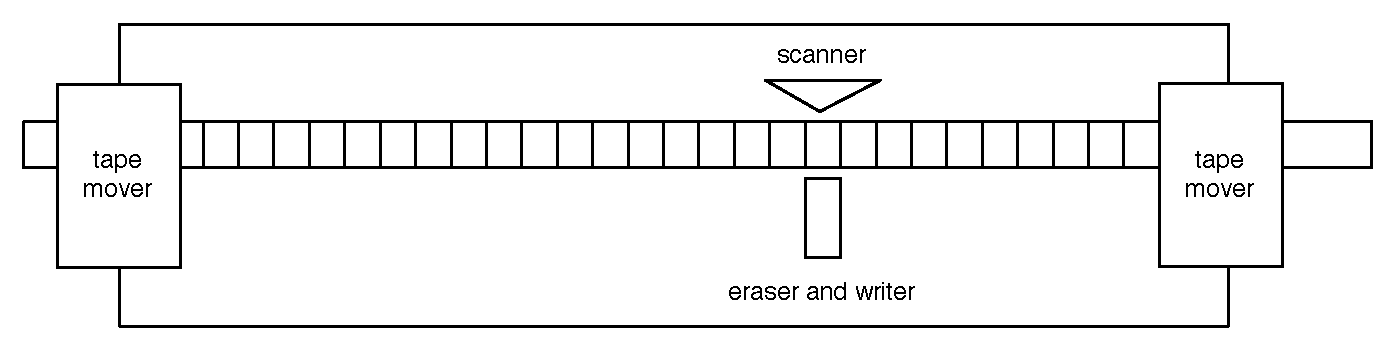
\includegraphics[width=0.9\textwidth]{turingmachine}
\caption{A Turing machine.}
\label{fig:machine}
\end{figure}


\begin{figure}
\centering
\subbottom[Turing Machine 1\label{fig:tm:tm1}]{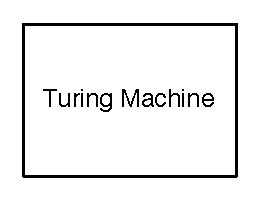
\includegraphics[width=0.2\textwidth]{block}}
\subbottom[Turing Machine 2\label{fig:tm:tm2}]{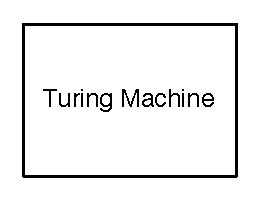
\includegraphics[width=0.2\textwidth]{block}}
\subbottom[Turing Machine 3\label{fig:tm:tm3}]{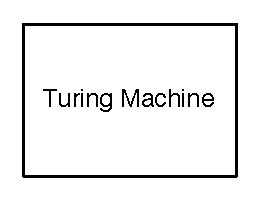
\includegraphics[width=0.2\textwidth]{block}}
\subbottom[Turing Machine 4\label{fig:tm:tm4}]{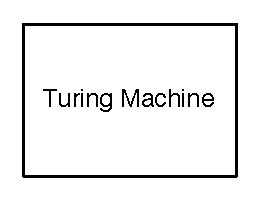
\includegraphics[width=0.2\textwidth]{block}}
\caption{Plots of four Turing machines}
\label{fig:tm}
\end{figure}




\section{Packages}
These packages might be helpful for writing your thesis:

\begin{description}
	\item[\texttt{caption}] to adjust the look of your captions
	\item[\texttt{glossaries}] for creating glossaries (also list of symbols)
	\item[\texttt{makeidx}] for indexes and the back of your document
	\item[\texttt{algorithm, algorithmicx, algpseudocode}] for adding algorithms to your document
\end{description}
%% !TEX root = ../Thesis.tex
\chapter{Conclusion}
This is a short conclusion on the thesis template documentation. If you have any comments or suggestions for improving the template, if you find any bugs or problems, please contact me. 

\vspace{2cm}

Good luck with your thesis!
%\input{./Chapters/Chapter4}
%\input{./Chapters/Chapter5}
%\input{./Chapters/Chapter6}
%\input{./Chapters/Chapter7}
%% ----------------------------------------------------------------
%\thesisappendix
\thesisbib
%\begin{appendices}
%	% !TEX root = ../Thesis.tex
\chapter{Mathematical tools}
\section{Power Iterations}
\label{sec:powerIterations}

Power iteration (also called power method) is a iteratively method, 
which approximates the biggest eigenvalue of a diagonalizable matrix $A$.

The algorithm starts with a random vector $b_0$ or an approximation of the dominant eigenvector.

\begin{equation}
    \label{eq:powerIterations}
    b_{k+1} = \frac{Ab_k}{||Ab_k||}
\end{equation}

\textbf{TODO:convergence if there is only one largest eigenvalue and if b0 is not orthogonal to the eigenvector associated with the largest eigenvalue.}

The algorithm not necessarily converges. The algorithm will converge, if $A$ has an eigenvalue strictly grater than its other eigenvalues
and the initial vector $b_0$ has a component in direction of an eigenvector, associated with the dominant eigenvector.

\section{Folded spectrum Method}

\textbf{TODO: I don't know what is the Hamiltonian matrix, so either you define it or don't talk about it. 
You can also introduce the folded spectrum just as a way to recover the eigenvector associated with a known eigenvalue. Epsilon often refers to a very small scalar.}


\label{sec:FoldedSpectrumMethod}
Calculation of eigenvalues and eigenvectors of a given Hamiltonian matrix $H$ 
is a fundamental mathematical problem. Often, we are interested in just the smallest 
values, which can be efficiently computed. But if we are interested in selected values,
this can be hard. $H$ is needed to be diagonalized (bring matrix $H$ into diagonal form) 
which is computationally expensive and for big matrices impossible.

Currently, the best way to solve such problems is the Folded spectrum (FS)\cite{foldedSpectrumMethod} method,
which iteratively solves the problem. During calculation, the eigenvalue spectrum will be folded around a reference 
value $\epsilon$.

\begin{equation}
    \label{eq:foldedSpectrumMethod}
    v^{t+1} = v^t - \alpha (H - \epsilon I )^2 v^t ,
\end{equation}

with $0 < \alpha < 1$. When $t \rightarrow \infty$, then $v^{\infty}$ will be the 
eigenvector with respect to the reference value $\epsilon$.


\section{Wasserstein metric}
\label{sec:wasserstein-metric}
\textbf{TODO: the difference between Wasserstein and KL divergence for instance is that it is defined (the value is finite) even if the two distributions have not the same support. }


The Wasserstein metric is a distance measure between two probability distributions and it is used in ML as a loss function\cite{learningWithWasserstein}. 
Intuitively, it can can be understood as the minimum cost to transfer the mass of one distribution to the other.
Therefore, it is also known as the \textit{earth mover's distance}.

As \citet{wassersteinGAN} could show, ordinary distance measures like \textit{Total Variation}, \textit{Kullback-Leibler divergence}
and \textit{Jensen-Shannon divergence} are not sensible when learning with distributions supported by manifolds
On the contrary, Wasserstein metric does a good job as loss function in such scenarios.


\section{Fourier Transform}
\textit{Fourier Analysis} is the overall field of study, which deals with representing (or approximating) functions as 
sums of trigonometric functions. When the function is defined in such a way, we are talking from the \textit{Fourier Domain}.

\textit{Fourier transform} (FT) is the way of transforming signals to the Fourier Domain, which is popular in ML.
Basically, with the Fourier transform, a signal can be decomposed to a \textit{Fourier series}, which consists of many weighted sinusoids. 

\paragraph{Fourier-slice theorem}
The Fourier-slice theorem \cite{fourierSliceTheorem} in 3D is defined as follows:

\begin{equation}
    \label{eq:Fourrier-slice}
    F_2 P_2 = S_2 F_3,
\end{equation}

where $F2$ and $F3$ are FTs in 2D and 3D respectively, P2 is a projection operator ($P_2 : 3D \rightarrow 2D$) and $S2$ is the restriction operator.

As pointed out by \cite{cryoEmMath},
the Fourier-slice theorem is the foundation of the reconstruction problem in computerized tomography (CT), which will be explained in section~\ref{sec:reconstructionProblemCT}.
It states, that the 2D FT of the tomographic projection is the same as the 3D FT restricted to a 2D plane through the origin.
Basically, for the CT reconstruction problem, acquiring samples from known viewing directions is the same 
as sampling the 3D Fourier-space. This concept is exploited by the filter BackProjection algorithms, see section~\ref{sec:filterBackProjection}.

\section{Radon Transform}
The radon transform\cite{radonTransform} is the main mathematically concept of tomographic reconstruction.

It is an integral transformation of a function $f(x,y)$, which is defined on the plane. In tomographic reconstruction
the function $f$ will be the observed tomographic image.
The radon transform then transforms $f$ to a function $Rf$, which corresponds to the line integral of the line defined by 
the two parameters $\theta$ and $s$, where $\theta$ is a angle and $s$ the distance to the origin.

In Figure~\ref{fig:phantom_theta45} and Figure~\ref{fig:phantom_theta45_s14} on can see two plots of different
values for $\theta$ and $s$, where $f(x,y)$ is the Shepp-Logan phantom. The complete $R(\theta=45, s=0)x$, 
which is also called \textit{sinogram}, can be see in Figure~\ref{fig:phantom_sinogram}

\begin{figure}[H]
    \centering
    \subbottom[Radon Transform  $R(\theta=45, s=0)x$\label{fig:phantom_theta45}]{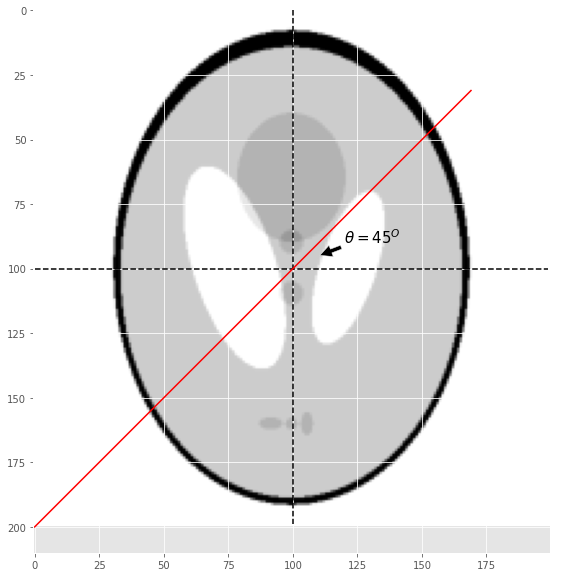
\includegraphics[width=0.3\textwidth]{phantom_theta45.png}}
    \subbottom[Radon Transform  $R(\theta=45, s=14.14)x$\label{fig:phantom_theta45_s14}]{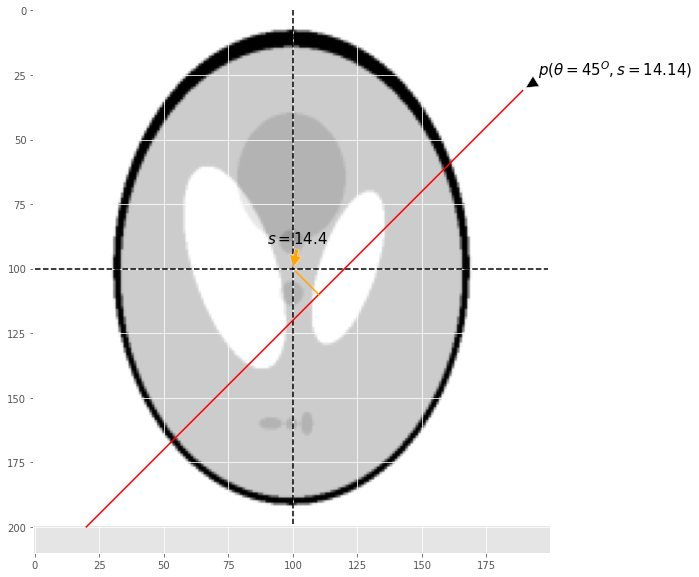
\includegraphics[width=0.3\textwidth]{phantom_theta45_s14.png}}
    \subbottom[Shepp–Logan phantom sinogram of $R(\theta=45, s=0)x$\label{fig:phantom_sinogram}]{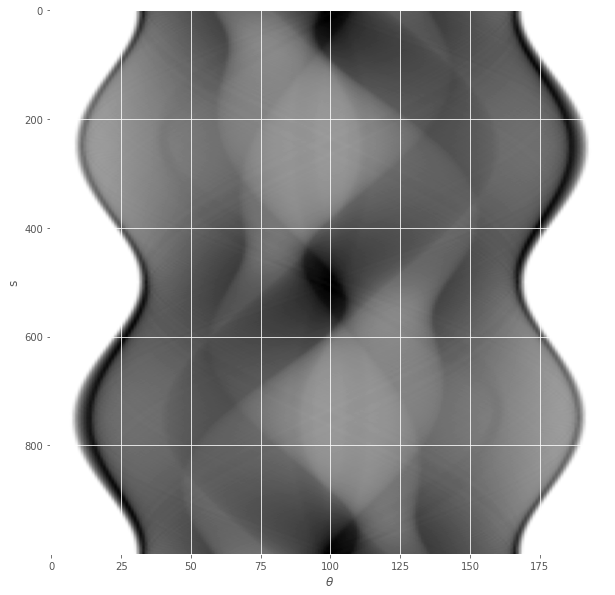
\includegraphics[width=0.3\textwidth]{phantom_sinogram.png}}
    \caption{Examples, where the original object $x$ is the Shepp-Logan phantom.}
\end{figure} 
%\end{appendices}
%% ----------------------------------------------------------------
%\thesisback
%\iflanguage{english}
%  {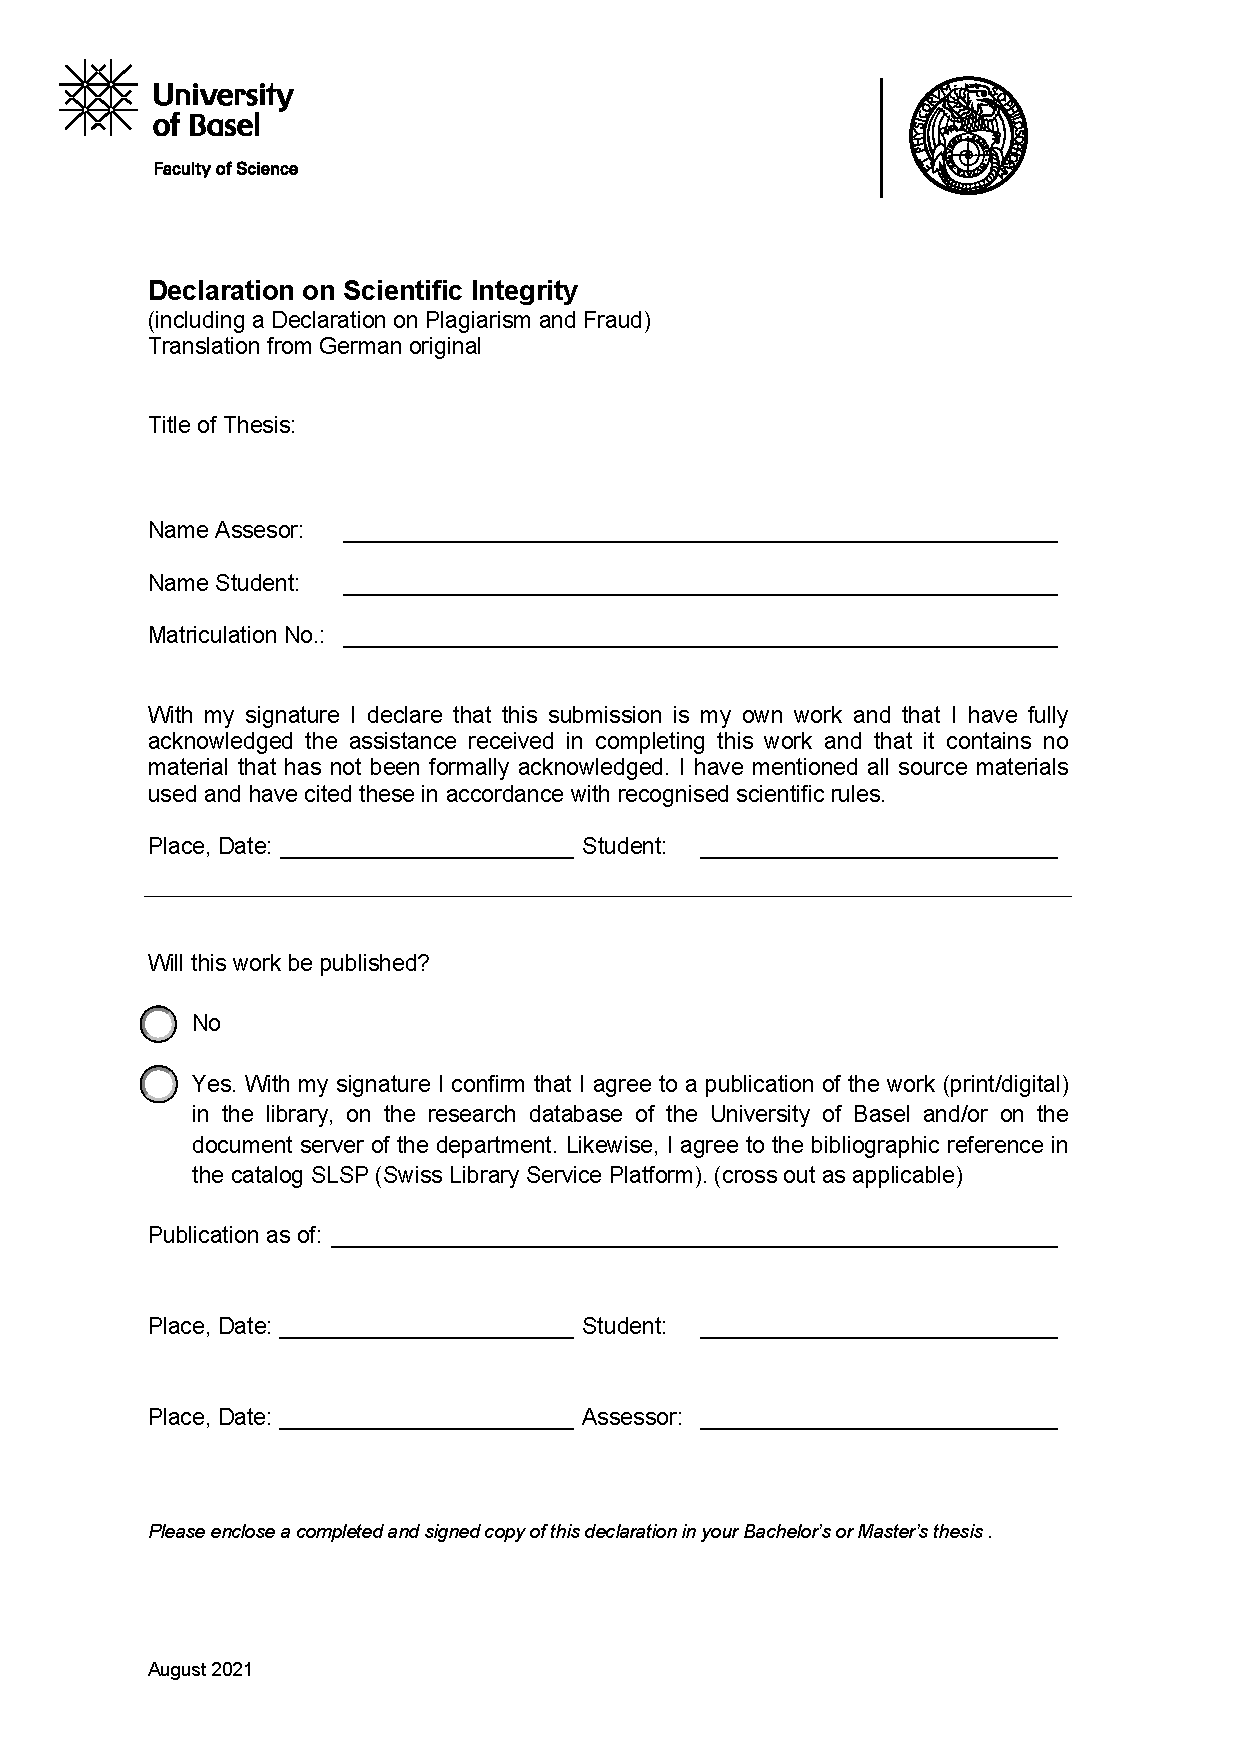
\includepdf{./Back/wissensch_Redlichkeit_E_Aug_21.pdf}}
%  {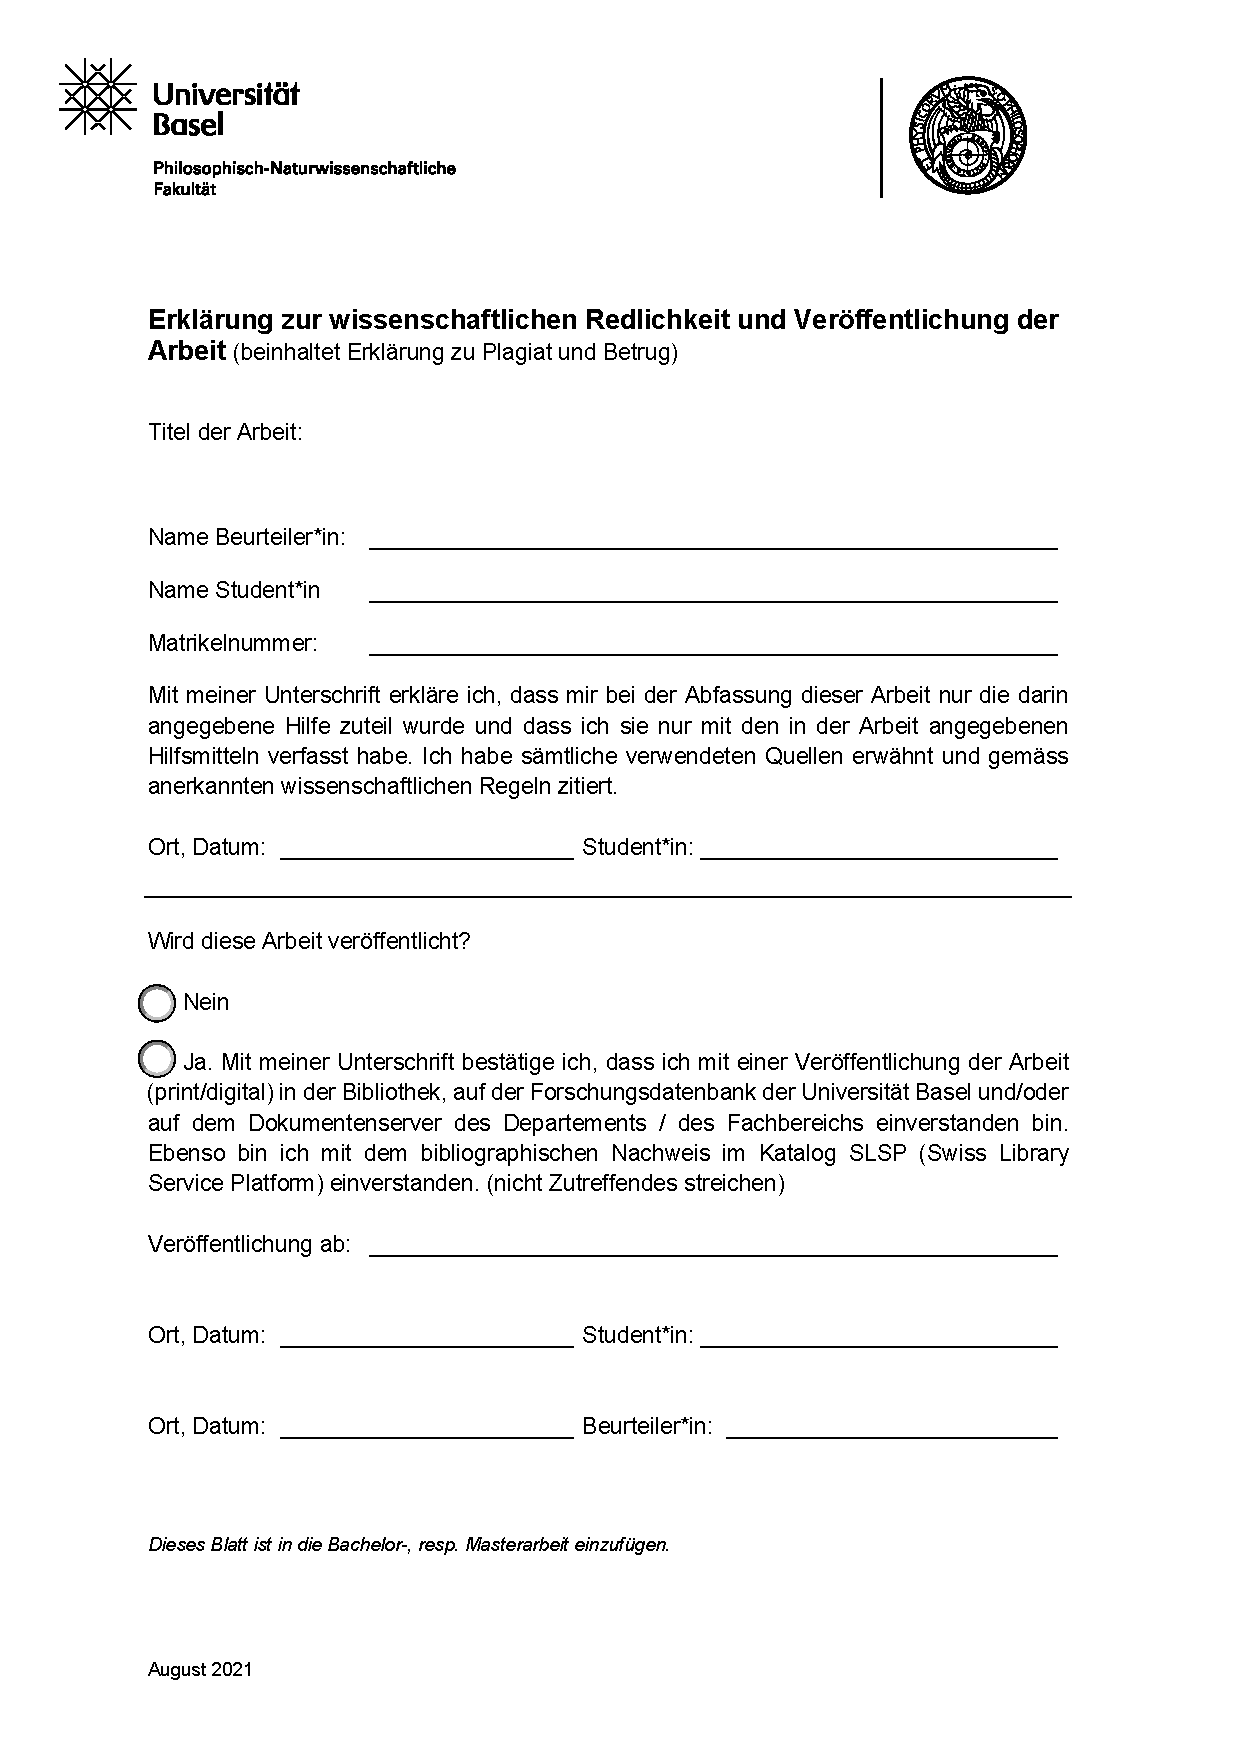
\includepdf{./Back/wissensch_Redlichkeit_D_Aug_21.pdf}}
%% ----------------------------------------------------------------
\end{document}
%% ----------------------------------------------------------------
